\section{PROJECT SIZE, COST AND EFFORT ESTIMATION}
This section provides some estimations on the expected size, cost and required effort of the PowerEnJoy project.

For the size estimation part we will use the Function Points approach, considering all the main PowerEnJoy functionalities and estimating the correspondent amount of lines of code to be written in Java. 

For the cost and effort estimation we will instead rely on the COCOMO approach, using as initial guidance the amount of lines of code computed with the FP approach.

\subsection{Size estimation: Function Points}
The Function Points approach provides an estimation of a project size taking as inputs the amount of functionalities to be developed and their complexity.

The complexity is evaluated based on the characteristics of the application and described in the following table:

\begin{figure}[H]
	\centering
	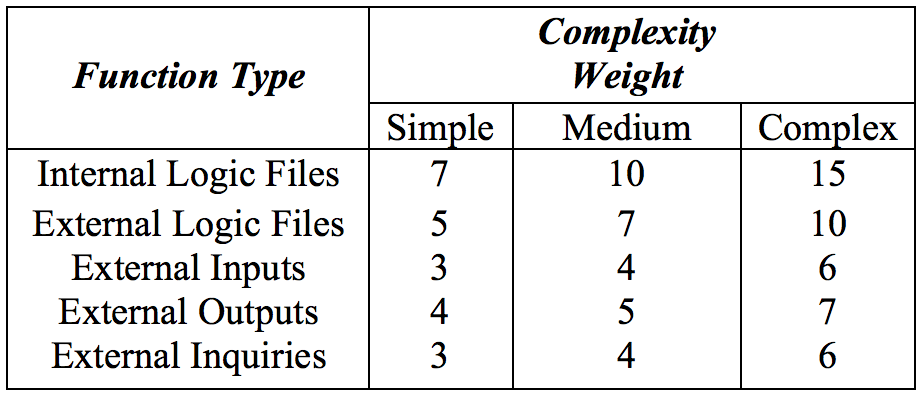
\includegraphics[width=12cm]{ComplexityWeights}
	\caption{UFP Complexity Weights}
\end{figure}
\newpage
\subsubsection{Internal Logic Files (ILFs)}
In this paragraph we analyze in details the various ILFs we have identified.

First of all, the system has to store information about users, registered users and employees. These data are condensed in a three-level structure. The first level holds id, first name, surname, username, password, driver license code and province of birth as strings, together with email address, card number and card code as contact information. A secondary table contains the location coordinates (as <latitude, longitude> pairs) necessary to identify the location of the registered user. A third table contains all the reservations related to the registered user.

As for the cars, they are stored using a three-level structure. The first level of the structure holds plate number, brand and model of the car as strings. It also stores the car’s status (reserved, broken, blocked, ignited, plugged, with low battery), number of active weight sensors, number of open doors, battery level and number of seats. A secondary table contains the location coordinates (as <latitude, longitude> pairs) necessary to identify the car's location. A third table contains the information related to the car's screen, such as price, total price, hours, minutes and percentage.

Reservations are stored in a dedicated table that holds all the information about the registered user who booked them, the reservation code, the starting and ending time and the reserved car.

Rides are also stored in a dedicated table with a similar structure, the only difference being the absence of the reservation code and the presence of an extra field for the total price.

Finally, the system keeps a list of safe areas, identified by a location and an attribute that indicates whether the safe area is special or not.

\begin{table}[H]
	\centering
	\begin{tabular}{| m{3cm} | m{2.5cm} | m{1cm} |}
		\hline
		\textbf{ILF} & \textbf{Complexity} & \textbf{FPs}\\
		\hline
		User & Complex & 15\\
		Registered User & Complex & 15\\
		Employee & Simple & 7\\
		Car & Complex & 15\\
		Reservation & Medium & 10\\
		Ride & Medium & 10\\
		Safe Area & Simple & 7\\
		\hline
		\multicolumn{2}{|c|}{Total} & 79\\
		\hline
	\end{tabular}
\end{table}

\subsubsection{External Logic Files (ELFs)}
In this paragraph we present the ELFs we have identified, which are homogeneous set of data used by the application but generated by other applications.
The only EIF of our system is the interface of a Mapping Service we use for:
\begin{itemize}
	\item Show the location of all PowerEnJoy cars in a certain geographical region.
	\item Given an address, get the correspondent pair of coordinates (reverse geocoding).
	\item Retrieve the graphical representation of the city map to be displayed on the car's screen.
\end{itemize}

\begin{table}[H]
	\centering
	\begin{tabular}{| m{4cm} | m{2.5cm} | m{1cm} |}
		\hline
		\textbf{ELF} & \textbf{Complexity} & \textbf{FPs}\\
		\hline
		Cars location retrieval & Medium & 7\\
		Reverse geocoding & Medium & 7\\
		Map data retrieval & Medium & 7\\
		\hline
		\multicolumn{2}{|c|}{Total} & 21\\
		\hline
	\end{tabular}
\end{table}

\subsubsection{External Inputs (EIs)}
PowerEnJoy supports many kind of interactions with different categories of users.

In this paragraph we are going to summarize the impact of the offered features, grouping them by user category.
\subsubsection*{Users}
\begin{itemize}
	\item \textbf{Registration} and \textbf{First login}: this operation has a \textit{high} complexity, as it involves a lot of components (Notification Manager, Registration Manager and Account Generator).
\end{itemize}

\subsubsection*{Registered User}
\begin{itemize}
	\item \textbf{Login/Logout/Manage personal information}: these are \textit{simple} operations that involve only the Account Manager.
	\item \textbf{Make reservation}: this operation has a \textit{high} complexity, as it involves a lot of components (Account Manager, Reservation Manager, Car Manager and Reservation Generator).
	\item \textbf{Report issue}: this operation has a \textit{medium} complexity, as it involves Account Manager, Reservation Manager and Car Manager.
	\item \textbf{Cancel current reservation}: this operation has a \textit{medium} complexity, as it involves Account Manager, Reservation Manager and Car Manager.
\end{itemize}

\subsubsection*{Employee}
\begin{itemize}
	\item \textbf{Login/Logout}: these are \textit{simple} operations that involve only the Account Manager.
	\item \textbf{Manage car information}: this operation has a \textit{simple} complexity since it involves only the Car Manager.
\end{itemize}

\begin{table}[H]
	\centering
	\begin{tabular}{| m{5.5cm} | m{2.5cm} | m{1cm} |}
		\hline
		\textbf{EI} & \textbf{Complexity} & \textbf{FPs}\\
		\hline
		Registration and First login & Complex & 6\\
		Login & Simple & 3\\
		Logout & Simple & 3\\
		Manage personal information & Simple & 3\\
		Make reservation & Complex & 6\\
		Report issue & Medium & 4\\
		Cancel current reservation & Medium & 4\\
		Manage car information & Simple & 3\\
		\hline
		\multicolumn{2}{|c|}{Total} & 32\\
		\hline
	\end{tabular}
\end{table}

\subsubsection{External Inquiries (EQs)}
As specified by the FP guidelines, an inquiry is essentially a data retrieval request performed by a user.

PowerEnJoy supports a few interactions of this type that do not require complex computations:
\begin{itemize}
	\item A registered user can retrieve his/her reservations history.
	\item A registered user can view his/her profile.
	\item A registered user can retrieve the active promotions.
\end{itemize}

\begin{table}[H]
	\centering
	\begin{tabular}{| m{5.2cm} | m{2.5cm} | m{1cm} |}
		\hline
		\textbf{EQ} & \textbf{Complexity} & \textbf{FPs}\\
		\hline
		Retrieve reservations history & Simple & 3\\
		View profile & Simple & 3\\
		Retrieve active promotions & Simple & 3\\
		\hline
		\multicolumn{2}{|c|}{Total} & 9\\
		\hline
	\end{tabular}
\end{table}

\subsubsection{External Outputs (EOs)} 
As part of its normal behavior, PowerEnJoy occasionally needs to communicate with the user outside the context of an inquiry. These occasions are:
\begin{itemize}
	\item Notify a user that he/she has received a password via email.
	\item Notify a registered user that more than ten minutes have passed since he/she parked the car in a non-safe area.
	\item Notify a registered user that his/her report on a car issue has been received.
\end{itemize}

\begin{table}[H]
	\centering
	\begin{tabular}{| m{5.3cm} | m{2.5cm} | m{1cm} |}
		\hline
		\textbf{EO} & \textbf{Complexity} & \textbf{FPs}\\
		\hline
		Receive password notification & Simple & 4\\
		Timeout notification & Simple & 4\\
		Report issue notification & Simple & 4\\
		\hline
		\multicolumn{2}{|c|}{Total} & 12\\
		\hline
	\end{tabular}
\end{table}

\subsubsection{Overall estimation}
The following table summarizes the results of our estimation activity:

\begin{table}[H]
	\centering
	\begin{tabular}{| m{3.8cm} | m{1.2cm} |}
		\hline
		\textbf{Function type} & \textbf{Value} \\
		\hline
		Internal Logic Files & 79\\
		External Logic Files & 21\\
		External Inputs & 32\\
		External Inquiries & 9\\
		External Outputs & 12\\
		\hline
		Total & 153\\
		\hline
	\end{tabular}
\end{table}

Considering Java as the development language, the conversion multiplier from function points to SLOC is 53.
We can thus estimate the total number of lines of code:

\begin{table}[H]
	\centering
	\begin{tabular}{| m{13cm} |}
		\hline
		SLOC = 153 * 53 = 8109\\
		\hline
	\end{tabular}
\end{table}

\subsection{Cost and effort estimation: COCOMO II}
In this paragraph we present the estimation of cost and effort needed to develop the PowerEnJoy application, by using the COCOMO II approach.

\subsubsection{Scale Drivers}
In order to evaluate the values of the scale drivers, we refer to the following official COCOMO II table:

\begin{table}[H]
	\centering
	\begin{tabular}{| m{1.6cm} | m{1.8cm} | m{1.7cm} | m{1.7cm} | m{1.5cm} | m{1.5cm} | m{1.8cm} | }
		\hline
		\textbf{Scale Factors} & \textbf{Very Low} & \textbf{Low} & \textbf{Nominal} & \textbf{High} & \textbf{Very High} & \textbf{Extra High} \\
		\hline
		\textbf{PREC \[SF_j\]} & thoroughly unprecedented 6.20 & largely unprecedented 4.96 & somewhat unprecedented 3.72 & generally familiar 2.48 & largely familiar 1.24 & thoroughly familiar 0.00 \\
		\hline
		\textbf{FLEX \[SF_j\]} & rigorous 5.07 & occasional relaxation 4.05 & some relaxation 3.04 & general conformity 2.03 & some conformity 1.01 & general goals \newline 0.00 \\
		\hline
		\textbf{RESL \[SF_j\]} & little (20\%) 7.07 & some (40\%) 5.65 & often (60\%) 4.24 & generally (75\%) 2.83 & mostly (90\%) 1.41 & full (100\%) 0.00 \\
		\hline
		\textbf{TEAM \[SF_j\]} & very difficult interactions 5.48 & some difficult interactions 4.38 & basically cooperative interactions 3.29 & largely cooperative 2.19 & highly cooperative 1.10 & seamless interactions 0.00 \\
		\hline
		\textbf{PMAT \[SF_j\]} & Level 1 \newline Lower 7.80 & Level 1 \newline Upper 6.24 & Level 2 \newline 4.68 & Level 3 \newline 3.12 & Level 4 \newline 1.56 & Level 5 \newline 0.00 \\
		\hline
	\end{tabular}
\end{table}
\newpage
A brief description for each scale driver:
\begin{itemize}
	\item \textbf{Precedentedness}, that reflects the previous experience of our team with the development of this type projects. Since we have some experience in software design but most of the notions required in this project are new to us, the precedentedness value is low.
	\item \textbf{Development Flexibility}, that reflects the degree of flexibility in the development process with respect to the external specifications and requirements. Since there are very strict requirements on the functionalities but nothing specific is stated regarding the technology to be used, this value will be low.
	\item \textbf{Risk Resolution}, that reflects the level of awareness and reactiveness with respect to risks. The risk analysis we performed is quite specific, so the value will be set to high.
	\item \textbf{Team Cohesion}, that is an indicator of how well the team members know each other and work together in a cooperative way. Since the cohesion and communication among the two of us is optimal, the value is very high.
	\item \textbf{Process Maturity}, that is the process maturity of the organization. Although we had some problems during the development of the project, the goals have been successfully achieved. Since this is our first project of this kind, this value is set to level 3.
\end{itemize}

The result of our evaluation is the following:
\begin{table}[H]
	\centering
	\begin{tabular}{| m{5.8cm} | m{1.8cm} | m{1.2cm} |}
		\hline
		\textbf{Scale Driver} & \textbf{Factor}& \textbf{Value} \\
		\hline
		Precedentedness (PREC) & Low & 4.96 \\
		Development flexibility (FLEX) & Low & 4.05 \\
		Risk resolution (RESL) & High & 2.83 \\
		Team cohesion (TEAM) & Very high & 1.10 \\
		Process maturity (PMAT) & Level 3 & 3.12 \\
		\hline
		\multicolumn{2}{|c|}{Total} & 16.06\\
		\hline
	\end{tabular}
\end{table}

\subsubsection{Cost Drivers}
\subsubsection*{Required Software Reliability (RELY)}
Since the system represents the only way to reserve electric cars in the city, a malfunctioning could lead to significant financial losses. For this reason, the RELY cost driver is set to high.

\begin{table}[H]
	\centering
	\begin{tabular}{| m{1.8cm} | m{1.8cm} | m{1.7cm} | m{1.7cm} | m{1.3cm} | m{1.3cm} | m{1cm} | }
		\hline
		\multicolumn{7}{|c|}{ \textbf{RELY Cost Driver} } \\
		\hline
		\hline
		\textbf{RELY Descriptors} & slight inconvenience & low, easily recoverable losses & moderate, easily recoverable losses & high financial loss & risk to human life & \\
		\hline
		\textbf{Rating Levels} & Very Low & Low & Nominal & High & Very High & Extra High \\
		\hline
		\textbf{Effort Multipliers} & 0.82 & 0.92 & 1.00 & 1.10 & 1.26 & n/a \\ 
		\hline
	\end{tabular}
\end{table}

\subsubsection*{Data Base Size (DATA)}
This measure considers the effective size of our database. We don't have the ultimate answer, but our estimation given the tables and fields we have is to reach a 3MB database. Since it is distributed over 8.000 SLOC, the ratio D/P (measured as testing DB bytes/program SLOC) is 393, resulting in the DATA cost driver being high.

\begin{table}[H]
	\centering
	\begin{tabular}{| m{1.8cm} | m{0.8cm} | m{1.4cm} | m{2.5cm} | m{2.7cm} | m{1.5cm} | m{0.9cm} | }
		\hline
		\multicolumn{7}{|c|}{ \textbf{DATA Cost Driver} } \\
		\hline
		\hline
		\textbf{DATA Descriptors} & & \(\frac{D}{P} < 10\)  & \(10 \leq \frac{D}{P} < 10^2\) & \( 10^2 \leq \frac{D}{P} < 10^3\) & \(\frac{D}{P}\geq 10^3\) & \\
		\hline
		\textbf{Rating Levels} & Very Low & Low & Nominal & High & Very High & Extra High \\
		\hline
		\textbf{Effort Multipliers} & n/a & 0.90 & 1.00 & 1.14 & 1.28 & n/a \\ 
		\hline
	\end{tabular}
\end{table} 

\subsubsection*{Product Complexity (CPLX)}
Set to nominal according to the COCOMO II rating scale.

\begin{table}[H]
	\centering
	\begin{tabular}{| m{1.8cm} | m{1.7cm} | m{0.8cm} | m{1.5cm} | m{0.9cm} | m{1.8cm} | m{2cm} | }
		\hline
		\multicolumn{7}{|c|}{ \textbf{CPLX Cost Driver} } \\
		\hline
		\hline
		\textbf{Rating Levels} & Very Low & Low & Nominal & High & Very High & Extra High \\
		\hline
		\textbf{Effort Multipliers} & 0.73 & 0.87 & 1.00 & 1.17 & 1.34 & 1.74 \\ 
		\hline
	\end{tabular}
\end{table}
\newpage
\subsubsection*{Developed for Reusability (RUSE)}
In our case, the reusability requirements are limited in scope to the project itself, so the RUSE cost driver is set to nominal.

\begin{table}[H]
	\centering
	\begin{tabular}{| m{1.8cm} | m{0.8cm} | m{0.8cm} | m{1.5cm} | m{1.6cm} | m{1.5cm} | m{2.8cm} | }
		\hline
		\multicolumn{7}{|c|}{ \textbf{RUSE Cost Driver} } \\
		\hline
		\hline
		\textbf{RUSE Descriptors} & & none  & across project & across program & across product line & across multiple product lines \\
		\hline
		\textbf{Rating Levels} & Very Low & Low & Nominal & High & Very High & Extra High \\
		\hline
		\textbf{Effort Multipliers} & n/a & 0.95 & 1.00 & 1.07 & 1.15 & 1.24 \\ 
		\hline
	\end{tabular}
\end{table} 

\subsubsection*{Documentation Match to Life-Cycle Needs (DOCU)}
This parameter is evaluated in terms of the suitability of the project's documentation to its life-cycle needs. In our case, every life-cycle need presented in the documentation is covered, so the DOCU cost driver is set to nominal.

\begin{table}[H]
	\centering
	\begin{tabular}{| m{1.8cm} | m{1.9cm} | m{1.7cm} | m{1.6cm} | m{1.6cm} | m{1.8cm} | m{0.9cm} | }
		\hline
		\multicolumn{7}{|c|}{ \textbf{DOCU Cost Driver} } \\
		\hline
		\hline
		\textbf{DOCU Descriptors} & Many life-cycle needs uncovered & Some life-cycle needs uncovered & Right-sized to life-cycle needs & Excessive for life-cycle needs & Very excessive for life-cycle needs & \\
		\hline
		\textbf{Rating Levels} & Very Low & Low & Nominal & High & Very High & Extra High \\
		\hline
		\textbf{Effort Multipliers} & 0.81 & 0.91 & 1.00 & 1.11 & 1.23 & n/a \\ 
		\hline
	\end{tabular}
\end{table} 
\newpage
\subsubsection*{Execution Time Constraint (TIME)}
This is a measure of the execution time constraint imposed upon a software system. The rating is expressed in terms of the percentage of available execution time expected to be used by the system or subsystem consuming the execution time resource. As PowerEnJoy is a quite complex piece of software, we expect that its CPU usage will be high.

\begin{table}[H]
	\centering
	\begin{tabular}{| m{1.8cm} | m{0.8cm} | m{0.8cm} | m{1.8cm} | m{1.8cm} | m{1.8cm} | m{1.8cm} | }
		\hline
		\multicolumn{7}{|c|}{ \textbf{TIME Cost Driver} } \\
		\hline
		\hline
		\textbf{TIME Descriptors} & & & \(\leq\) 50\% \newline use of \newline available execution time & 70\% use of available execution time & 85\% use of available execution time & 95\% use of available execution time\\
		\hline
		\textbf{Rating Levels} & Very Low & Low & Nominal & High & Very High & Extra High \\
		\hline
		\textbf{Effort Multipliers} & n/a & n/a & 1.00 & 1.11 & 1.29 & 1.63 \\ 
		\hline
	\end{tabular}
\end{table} 

\subsubsection*{Main Storage Constraint (STOR)}
This rating represents the degree of main storage constraint imposed on a software system or subsystem. As current disk drives can easily contain several terabytes of storage, this value is set to nominal.

\begin{table}[H]
	\centering
	\begin{tabular}{| m{1.8cm} | m{0.8cm} | m{0.8cm} | m{1.8cm} | m{1.8cm} | m{1.8cm} | m{1.8cm} | }
		\hline
		\multicolumn{7}{|c|}{ \textbf{STOR Cost Driver} } \\
		\hline
		\hline
		\textbf{STOR Descriptors} & & & \(\leq\) 50\% \newline use of \newline available execution time & 70\% use of available execution time & 85\% use of available execution time & 95\% use of available execution time\\
		\hline
		\textbf{Rating Levels} & Very Low & Low & Nominal & High & Very High & Extra High \\
		\hline
		\textbf{Effort Multipliers} & n/a & n/a & 1.00 & 1.05 & 1.17 & 1.46 \\ 
		\hline
	\end{tabular}
\end{table} 

\subsubsection*{Platform Volatility (PVOL)}
The client applications may require at least a major release once every six months in order to be aligned with the development cycle of the main mobile operating systems. For this reason, this parameter is set to nominal.

\begin{table}[H]
	\centering
	\begin{tabular}{| m{1.8cm} | m{0.8cm} | m{2.5cm} | m{1.5cm} | m{1.5cm} | m{1.5cm} | m{0.9cm} | }
		\hline
		\multicolumn{7}{|c|}{ \textbf{PVOL Cost Driver} } \\
		\hline
		\hline
		\textbf{PVOL Descriptors} & & Major change every 12 mo.; Minor change every 1 mo. & Major: 6 mo.; Minor: 2 wk. & Major: 2 mo.; Minor: 1 wk. & Major: 2 wk.; Minor: 2 days & \\
		\hline
		\textbf{Rating Levels} & Very Low & Low & Nominal & High & Very High & Extra High \\
		\hline
		\textbf{Effort Multipliers} & n/a & 0.87 & 1.00 & 1.15 & 1.30 & n/a \\ 
		\hline
	\end{tabular}
\end{table}

\subsubsection*{Analyst Capability (ACAP)}
Analysts are personnel who work on requirements, high-level design and detailed design. We think the analysis of the problem has been conducted in a thorough and complete way with respect to a potential real world implementation. For this reason, this parameter is set to high.

\begin{table}[H]
	\centering
	\begin{tabular}{| m{1.8cm} | m{1.6cm} | m{1.6cm} | m{1.6cm} | m{1.6cm} | m{1.6cm} | m{0.9cm} | }
		\hline
		\multicolumn{7}{|c|}{ \textbf{ACAP Cost Driver} } \\
		\hline
		\hline
		\textbf{ACAP Descriptors} & 15th \newline percentile & 35th \newline percentile & 55th \newline percentile & 75th \newline percentile & 90th \newline percentile & \\
		\hline
		\textbf{Rating Levels} & Very Low & Low & Nominal & High & Very High & Extra High \\
		\hline
		\textbf{Effort Multipliers} & 1.42 & 1.19 & 1.00 & 0.85 & 0.71 & n/a \\ 
		\hline
	\end{tabular}
\end{table}
\newpage
\subsubsection*{Programmer Capability (PCAP)}
The evaluation is based on our capability as a team rather than as individuals. Major factors which should be considered in the rating are ability, efficiency and thoroughness, and the ability to communicate and cooperate. We have not implemented the project, so this parameter is just an estimation; however we are fairly in our programming abilities, so we will set this parameter to high.

\begin{table}[H]
	\centering
	\begin{tabular}{| m{1.8cm} | m{1.6cm} | m{1.6cm} | m{1.6cm} | m{1.6cm} | m{1.6cm} | m{0.9cm} | }
		\hline
		\multicolumn{7}{|c|}{ \textbf{PCAP Cost Driver} } \\
		\hline
		\hline
		\textbf{PCAP Descriptors} & 15th \newline percentile & 35th \newline percentile & 55th \newline percentile & 75th \newline percentile & 90th \newline percentile & \\
		\hline
		\textbf{Rating Levels} & Very Low & Low & Nominal & High & Very High & Extra High \\
		\hline
		\textbf{Effort Multipliers} & 1.34 & 1.15 & 1.00 & 0.88 & 0.76 & n/a \\ 
		\hline
	\end{tabular}
\end{table}

\subsubsection*{Personnel Continuity (PCON)}
This parameter is set to nominal.

\begin{table}[H]
	\centering
	\begin{tabular}{| m{1.8cm} | m{1.6cm} | m{1.6cm} | m{1.6cm} | m{1.6cm} | m{1.6cm} | m{0.9cm} | }
		\hline
		\multicolumn{7}{|c|}{ \textbf{PCON Cost Driver} } \\
		\hline
		\hline
		\textbf{PCON Descriptors} & 48\%/year & 24\%/year & 12\%/year & 6\%/year & 3\%/year & \\
		\hline
		\textbf{Rating Levels} & Very Low & Low & Nominal & High & Very High & Extra High \\
		\hline
		\textbf{Effort Multipliers} & 1.29 & 1.12 & 1.00 & 0.90 & 0.81 &  \\ 
		\hline
	\end{tabular}
\end{table}
\newpage
\subsubsection*{Application Experience (APEX)}
The rating for this cost driver depends on the level of applications experience of the project team developing the software system. We have some experience in the development of Java applications, but we never tackled a Java EE system of this kind. For this reason we are going to set this parameter to low.

\begin{table}[H]
	\centering
	\begin{tabular}{| m{1.8cm} | m{2.2cm} | m{1.7cm} | m{1.5cm} | m{1.3cm} | m{1.3cm} | m{0.9cm} | }
		\hline
		\multicolumn{7}{|c|}{ \textbf{APEX Cost Driver} } \\
		\hline
		\hline
		\textbf{APEX Descriptors} & \(\leq\) 2 months & 6 months & 1 year & 3 years & 6 years & \\
		\hline
		\textbf{Rating Levels} & Very Low & Low & Nominal & High & Very High & Extra High \\
		\hline
		\textbf{Effort Multipliers} & 1.22 & 1.10 & 1.00 & 0.88 & 0.81 & n/a \\ 
		\hline
	\end{tabular}
\end{table}

\subsubsection*{Platform Experience (PLEX)}
We do not have any experience with the Java EE platform, but we have some previous experience with databases, user interfaces and server side development. For this reason, we are going to set this parameter to low.

\begin{table}[H]
	\centering
	\begin{tabular}{| m{1.8cm} | m{2.2cm} | m{1.7cm} | m{1.5cm} | m{1.3cm} | m{1.3cm} | m{0.9cm} | }
		\hline
		\multicolumn{7}{|c|}{ \textbf{PLEX Cost Driver} } \\
		\hline
		\hline
		\textbf{PLEX Descriptors} & \(\leq\) 2 months & 6 months & 1 year & 3 years & 6 years & \\
		\hline
		\textbf{Rating Levels} & Very Low & Low & Nominal & High & Very High & Extra High \\
		\hline
		\textbf{Effort Multipliers} & 1.19 & 1.09 & 1.00 & 0.91 & 0.85 & n/a \\ 
		\hline
	\end{tabular}
\end{table}
\newpage
\subsubsection*{Language and Tool Experience (LTEX)}
This is a measure of the level of programming language and software tool experience of the project team developing the software system. We do not have any experience with the Java EE language, but we have some previous experience with the development environment, so we are going to set this parameter to low.

\begin{table}[H]
	\centering
	\begin{tabular}{| m{1.8cm} | m{2.2cm} | m{1.7cm} | m{1.5cm} | m{1.3cm} | m{1.3cm} | m{0.9cm} | }
		\hline
		\multicolumn{7}{|c|}{ \textbf{LTEX Cost Driver} } \\
		\hline
		\hline
		\textbf{LTEX Descriptors} & \(\leq\) 2 months & 6 months & 1 year & 3 years & 6 years & \\
		\hline
		\textbf{Rating Levels} & Very Low & Low & Nominal & High & Very High & Extra High \\
		\hline
		\textbf{Effort Multipliers} & 1.20 & 1.09 & 1.00 & 0.91 & 0.84 & n/a \\ 
		\hline
	\end{tabular}
\end{table}

\subsubsection*{Use of Software Tools (TOOL)}
Our application environment is basic and moderately integrated, so we will set this parameter to nominal.

\begin{table}[H]
	\centering
	\begin{tabular}{| m{1.8cm} | m{1.1cm} | m{1.7cm} | m{1.6cm} | m{1.6cm} | m{2cm} | m{0.9cm} | }
		\hline
		\multicolumn{7}{|c|}{ \textbf{TOOL Cost Driver} } \\
		\hline
		\hline
		\textbf{TOOL Descriptors} & edit, code, debug & simple, frontend, backend CASE, little integration & basic life-cycle tools, moderately integrated & strong, mature life-cycle tools, moderately integrated & strong, mature, proactive life-cycle tools, well integrated with processes, methods, reuse &  \\
		\hline
		\textbf{Rating Levels} & Very Low & Low & Nominal & High & Very High & Extra High \\
		\hline
		\textbf{Effort Multipliers} & 1.17 & 1.09 & 1.00 & 0.90 & 0.78 & n/a \\ 
		\hline
	\end{tabular}
\end{table}

\subsubsection*{Multisite Development (SITE)}
This involves the assessment and judgement-based averaging of two factors: site collocation (from fully collocated to international distribution) and communication support (from surface mail and some phone access to full interactive multimedia). Since we live in the same city and we have collaborated relying hugely on wideband Internet services, we are going to set this parameter to high.

\begin{table}[H]
	\centering
	\begin{tabular}{| m{1.8cm} | m{1.1cm} | m{1.7cm} | m{1.5cm} | m{1.7cm} | m{2cm} | m{1.2cm} | }
		\hline
		\multicolumn{7}{|c|}{ \textbf{SITE Cost Driver} } \\
		\hline
		\hline
		\textbf{SITE Descriptors} & Inter- national & Multi-city and Multi-company & Multi-city or Multi-company & Same city or metro area & Same building or complex & Fully collocated\\
		\hline
		\textbf{SITE Communications Descriptors} & Some phone, mail & Individual phone, FAX & Narrow band email & Wideband electronic communication & Wideband elect. comm., occasional video conf. & Interac- tive multimedia\\
		\hline
		\textbf{Rating Levels} & Very Low & Low & Nominal & High & Very High & Extra High \\
		\hline
		\textbf{Effort Multipliers} & 1.17 & 1.09 & 1.00 & 0.90 & 0.78 & n/a \\ 
		\hline
	\end{tabular}
\end{table}
\newpage
\subsubsection*{Required Development Schedule (SCED)}
This rating measures the schedule constraint imposed on the project team developing the software. Although our efforts were well distributed over the available development time, the definition of all the required documentation took a consistent amount of time, especially for the requirement analysis and the design phases. For this reason, this parameter is set to high.

\begin{table}[H]
	\centering
	\begin{tabular}{| m{1.8cm} | m{1.5cm} | m{1.5cm} | m{1.5cm} | m{1.5cm} | m{1.8cm} | m{1cm} | }
		\hline
		\multicolumn{7}{|c|}{ \textbf{SCED Cost Driver} } \\
		\hline
		\hline
		\textbf{SCED Descriptors} & 75\% of nominal & 85\% of nominal & 100\% of nominal & 130\% of nominal & 160\% of nominal & \\
		\hline
		\textbf{Rating Levels} & Very Low & Low & Nominal & High & Very High & Extra High \\
		\hline
		\textbf{Effort Multipliers} & 1.43 & 1.14 & 1.00 & 1.00 & 1.00 & n/a \\ 
		\hline
	\end{tabular}
\end{table}

Overall, our results are expressed by the following table:
\begin{table}[H]
	\centering
	\begin{tabular}{| m{9.5cm} | m{1.8cm} | m{1.2cm} |}
		\hline
		\textbf{Cost Driver} & \textbf{Factor}& \textbf{Value} \\
		\hline
		Required Software Reliability (RELY) & High & 1.10 \\
		Data Base Size (DATA) & High & 1.14 \\
		Product Complexity (CPLX) & Nominal & 1.00 \\
		Developed for Reusability (RUSE) & Nominal & 1.00 \\
		Documentation Match to Life-Cycle Needs (DOCU) & Nominal & 1.00 \\
		Execution Time Constraint (TIME) & High & 1.11 \\
		Main Storage Constraint (STOR) & Nominal & 1.00 \\
		Platform Volatility (PVOL) & Nominal & 1.00 \\
		Analyst Capability (ACAP) & High & 0.85 \\
		Programmer Capability (PCAP) & High & 0.88 \\
		Personnel Continuity (PCON) & Nominal & 1.00 \\
		Application Experience (APEX) & Low & 1.10 \\
		Platform Experience (PLEX) & Low & 1.09 \\
		Language and Tool Experience (LTEX) & Low & 1.09 \\
		Use of Software Tools (TOOL) & Nominal & 1.00 \\
		Multisite Development (SITE) & High & 0.93 \\
		Required Development Schedule (SCED) & High & 1.00 \\
		\hline
		\multicolumn{2}{|c|}{Total} & 1.2655 \\
		\hline
	\end{tabular}
\end{table}

\subsubsection{Effort equation}
This final equation gives us the effort estimation measured in Person-Months (PM):

\begin{table}[H]
	\centering
	\begin{tabular}{| m{13cm} |}
		\hline
		\(PM = A * Size^E * \prod_{1 \leq i \leq n} EM_i \)\\ [0.6ex]
		\hline
	\end{tabular}
\end{table}

where:

\begin{table}[H]
	\centering
	\begin{tabular}{| m{13cm} |}
		\hline
		\textit{A} = 2.94 (This approximates a productivity constant in PM/ KSLOC (Person-Months/Kilo-Source Lines of Code)). \newline
		\textit{Size} = estimated size of the project in KSLOC (it can be deducted from UFP).\newline
  		\textit{EM} = Effort Multiplier (the method offers an approach to derive them from Cost Drivers).\newline
  		\(E = B + 0.01 * \sum_{1 \leq j \leq 5} SF_j = 0.91 + 0.01 * 16.06 = 0.91 + 0.1606 = 1.0706\)\\
		\hline
	\end{tabular}
\end{table}

With this parameters we can compute the effort value:

\begin{table}[H]
	\centering
	\begin{tabular}{| m{13cm} |}
		\hline
		\(PM = A * Size^E * \prod_{1 \leq i \leq n} EM_i = 2.94 * 8.109^{1.0706} * 1.2655= 56.957 \approx 57\)\\ [0.5ex]
		\hline
	\end{tabular}
\end{table}

\subsubsection{Schedule estimation}
Regarding the final schedule, we are going to use the following formula taken from COCOMO II manual:

\begin{table}[H]
	\centering
	\begin{tabular}{| m{13cm} |}
		\hline
		\(TDEV_{NS} = C * (PM_{NS})^F\)\\ [0.5ex]
		\hline
	\end{tabular}
\end{table}

Where:

\begin{table}[H]
	\centering
	\begin{tabular}{| m{13cm} |}
		\hline
		\(F = D + 0.2 * 0.01 * \sum_{j=1}^{5} SF_j = D + 0.2 * (E - B) = 0.28 + 0.2 * (1.0706 - 0.91) = 0.31212\) \newline
		\(PM = 56.957\) \newline
		\(TDEV_{NS} = 3.67 * 56.957^{ 0.31212} = 12.96\) months
		\\ [0.5ex]
		\hline
	\end{tabular}
\end{table}
